\cleardoublepage

% \newpage
% \thispagestyle{empty}
% \mbox{}

\chapter{Modelos de programación basados en paralelismo a nivel de tareas}
\label{ch:chapter3}

\section{Descripción general y estado del arte}

\section{OmpSs}

\subsection{Modelo de programación}

\subsection{Planificador de tareas}

\subsection{Ejemplo. Factorización de Cholesky}


\section{Adaptación de OmpSs a arquitecturas asimétricas (botlev)}
%%
\comentario{Título: No se si adaptación, o ampliación, o incorporación, o uso de
  OmpSs sobre asim, o ...} %%
Con el reciente auge de las arquitecturas asimétricas en el mundo HPC, el
equipo de desarrollo de OmpSs ha introducido un nuevo planificador
denominado \emph{Bottom level-aware scheduler} (Botlev)~\cite{botlev}
específico para este nuevo tipo de arquitecturas. Botlev recoge las ideas
de los planificadores tradicionales basados en arquitecturas heterogéneas,
distinguiendo únicamente dos tipos de nodos de cómputo (un nodo rápido
formado por los cores de tipo big, y un nodo de cómputo lento formado por
los cores de tipo LITTLE) y eliminando el
cálculo de los costes asociados a la transferencia de datos. \\
La principal idea que se encuentra detrás de Botlev es la de detectar en
tiempo de ejecución qué tareas pertenecen al camino crítico y cuáles no, y
obligar a que los cores rápidos sean los encargados de ejecutar las tareas
del camino crítico. Además, en caso de existir alguna tarea perteneciente
al camino crítico lista para ser ejecutada, esta tendrá preferencia sobre
el resto de tareas que también estén listas para ejecución.\\
El objetivo de garantizar que las tareas del camino crítico se ejecutan en
los cores rápidos cuanto antes es asegurarse que al ejecutar las tareas
críticas, estas liberarán dependencias con nuevas tareas que pasarán a
estar listas para ejecución, y así intentar conseguir que nunca haya cores
ociosos, lo cual disminuiría el rendimiento global de la aplicación. La
principal diferencia entre botlev y los planificadores tradicionales para
sistemas heterogéneos es que botlev toma las decisiones en tiempo dinámico
sin necesidad de conocer de antemano información sobre las tareas, o al
forma del árbol de dependencias.

Para determinar si una tarea pertenece al camino crítico o no en tiempo de
ejecución, botlev asigna una prioridad a cada tarea en el momento de la
inserción en el grafo de dependencias. Una vez que la tarea está lista para
ser ejecutada (es decir, cuando todas las tareas que tenían relación con la
tarea mediante el grafo de dependencias han finalizado su ejecución), se
realiza la decisión de qué core va a ejecutar la tarea en función de la
prioridad
asignada.\\
La prioridad de una tarea viene dada por un número entero positivo, el cuál
representa la longitud del camino más largo desde la tarea actual hasta una
tarea hoja del grafo de dependencias. Cuando una tarea es introducida en el
grafo de dependencias, se le asigna una prioridad 0 ya que la longitud del
camino más largo desde la tarea a un nodo hoja (ella misma) es 0. Además,
cuando una tarea se inserta en el TDG, se actualizan las prioridades de
todas las tareas predecesoras, ya que estas pueden haber cambiado. Por cada
tarea predecesora, se intenta aumentar la prioridad en 1 unidad (el camino
es un nodo más largo), siempre que no tuviera una prioridad mayor antes
(este es el caso de que la tarea pertenezca a un camino más largo en el que
la nueva tarea no esté involucrada). El proceso de actualización finaliza
cuando se actualiza la tarea raíz del árbol, o cuando se alcanza una tarea
que pertenece a otro camino más largo que el actual. En la
figura~\ref{s3:fig:botlev_tdg} se puede ver el camino crítico detectado
para una factorización de Cholesky sobre una matriz dividida en $8\times8$
bloques. Hay que destacar que esta forma de calcular el camino crítico
detecta las tareas que pertenecen al camino más largo, pero eso no implica
que sean aquellas que más van a retrasar la ejecución en caso de que no se
ejecuten de manera prioritaria. Para calcular esto, sería necesario conocer
de antemano las necesidades de cada tarea, o ir almacenando resultados
parciales de ejecución de manera dinámica para tomar decisiones en el
futuro.
%%
\comentario{La figura de las colas no se ve muy bien.} %%
\begin{figure}
  \centering
  
  \begin{subfigure}{.45\textwidth}
    \centering
    \setlength{\fboxsep}{5pt}
    \fbox{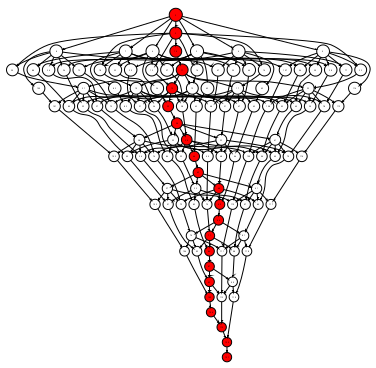
\includegraphics[width=.8\linewidth]{Figures/botlev-tdg.png}}
    \caption{Camino crítico en botlev para una factorización de Cholesky de
      $8\times8$ bloques.}
    \label{s3:fig:botlev_tdg}
  \end{subfigure}
  % Si se deja una línea en blanco, las coloca en vertical
  \begin{subfigure}{.45\textwidth}
    \centering
    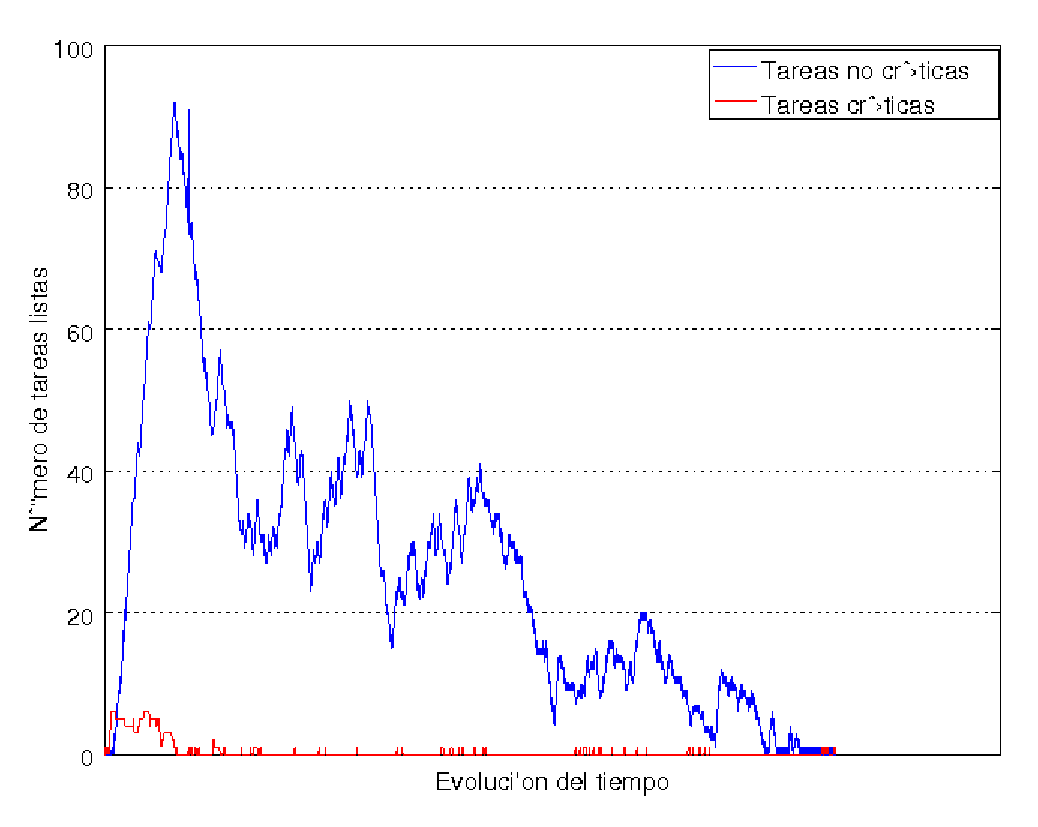
\includegraphics[width=1\linewidth]{Figures/botlev-colas.eps}
    \caption{Evolución del tamaño de las colas de tareas
      listas.\todo{agrandar texto}}
    \label{s3:fig:botlev_colas}
  \end{subfigure}  
  
  \caption{Cálculo de tareas críticas en Botlev y asignación a cores.}
  \label{s3:fig:botlev}
\end{figure}

Una tarea puede ser ejecutada cuando todas sus tareas predecesoras han
finalizado la ejecución. Cuando esto ocurre, Botlev inserta la tarea en una
cola de tareas pendientes para ir ejecutándolas en función de la prioridad
asignada, o en orden de insercción en caso de empate. Estas tareas son
asignadas a los diferentes cores según vayan finalizando la ejecución de
las tareas previas. Según la prioridad de la tarea, Botlev distingue dos
tipos de colas en las que insertar una tarea: la cola con las tareas
pertenecientes al camino crítico, y la cola con el resto de tareas. Una
tarea se considera que pertenece al camino crítico si posee una prioridad
mayor a cualquiera de las prioridades de las tareas anteriores, o si es
hija directa de una tarea que se ha considerado crítica y tiene una
prioridad de una unidad menor (es decir, es el siguiente nodo del camino
crítico). En la figura~\ref{s3:fig:botlev_colas} se puede ver la evolución
del tamaño de las colas para una factorización de Cholesky sobre una matriz
de $8\times8$ bloques. La línea azul muestra el número de tareas no
críticas listas para ser ejecutadas en función del momento de la ejecución
del problema, mientras que la línea roja muestra el
número de tareas críticas.

Cuando un core big finaliza la ejecución de una tarea, este ejecutará la
siguiente tarea de la cola de tareas críticas, mientras que un core LITTLE
ejecutará la primera tarea de la cola de tareas no críticas. De esta forma
se consigue asignar las tareas críticas a cores big, mientras que las
tareas no críticas serán ejecutadas por cores lentos. Para grafos de
dependencias muy anchos, como puede ser el asociado a una factorización de
Cholesky, el número de tareas críticas es mucho menor que el número de
tareas no críticas, dando lugar a que los cores rápidos estén la mayor
parte de tiempo ociosos. Para evitar esta situación, si un core big no
dispone de tareas críticas que ejecutar, ejecutará la siguiente tarea de la
lista de tareas no críticas. El robo de tareas en sentido contrario (es
decir, que los cores LITTLE ejecuten tareas críticas) es una parámetro
adicional que se puede seleccionar en tiempo de ejecución, pero que se
encuentra desactivado por defecto.





%-- Configuraciones para emacs --
%%% Local Variables:
%%% mode: latex
%%% TeX-master: "./principal.tex"
%%% End:
